\section*{Introduction}

A central concern of modern biology is understanding at the molecular level the chemical and physical mechanisms by which protein and nucleic acid macromolecules  perform essential cellular functions.  The operation of many such macromolecules requires that they work not as isolated molecules in solution but as components of dynamic molecular complexes that self-assemble and change structure and composition as they function.  For more than  two decades, scientists have successfully explored the molecular mechanisms of many such complex and dynamic systems using multi-wavelength single molecule fluorescence methods such as smFRET (single-molecule fluorescence resonance energy transfer) \cite{Roy2008-fo} and single-molecule co-localization methods like CoSMoS (co-localization single molecule spectroscopy) \cite{Larson2014-os, Van_Oijen2011-ig}.

CoSMoS is a technique to measure the kinetics of dynamic interactions between individual molecules.  The CoSMoS method has been used for elucidating the mechanisms of complex biochemical processes \textit{in vitro}. Examples include cell cycle regulation \cite{Lu2015-eu}, ubiquitination and proteasome-mediated protein degradation \cite{Lu2015-jq}, DNA replication \cite{Geertsema2014-bt,Ticau2015-ib}, transcription \cite{Zhang2012-no,Friedman2012-if,Friedman2013-sf}, micro-RNA regulation \cite{Salomon2015-kq}, pre-mRNA splicing \cite{Shcherbakova2013-bi, Krishnan2013-fy, Warnasooriya2014-ls}, ribosome assembly \cite{Kim2014-zc}, translation \cite{Wang2015-tt,Tsai2014-mi,OLeary2013-wo}, signal recognition particle-nascent protein interaction \cite{Noriega2014-vj}, and cytoskeletal regulation \cite{Smith2013-qj,Breitsprecher2012-mj}. 

In the simplest kind of CoSMoS experiment, dye-labeled protein or nucleic acid target molecules are immobilized on a slide surface and TIRF (total internal reflection fluorescence) microscopy is employed to detect co-localizations between those targets and other dye-labeled molecules that might bind those targets during a biochemical reaction. For example, Figure~\ref{fig1}A illustrates a CoSMoS experiment to measure %
\marginpar{
\vspace{.7cm} % adjust vertical position relative to text with \vspace{} - note that you can enter negative numbers to move margin caption up
\color{Gray} % this gives caption a grey color to set it apart from text body
\textbf{Figure \ref{fig1}. Example CoSMoS experiment.} % note that \ref{fig1} refers to the corresponding wrapfigure
(A) Experiment schematic. DNA target molecules labeled with a fluorescent dye are tethered to the microscope slide surface. RNA polymerase II (RNApII) binder molecules labeled with a different dye are present in solution. (B) Data collection and preprocessing. Preprocessing includes localization of target molecules in the blue channel, selection of on-target and off-target areas of interest (AOIs), registration of target and binder channels, and time-dependent drift correction. (C) On-target dataset. Data are time sequences of 14 x 14 pixel AOI images centered at each target molecule. Frames show on-target (e.g., frame 630) and off-target (e.g., frame 645) binding of RNApII molecules. (D) Off-target control dataset. Control data consists of images collected from randomly selected sites at which no target molecule is present. 
}
\begin{wrapfigure}[19]{l}{75mm}
% the number in [] of wrapfigure is optional and gives the number of text lines that should be wrapped around the text. Adjust according to your figures height
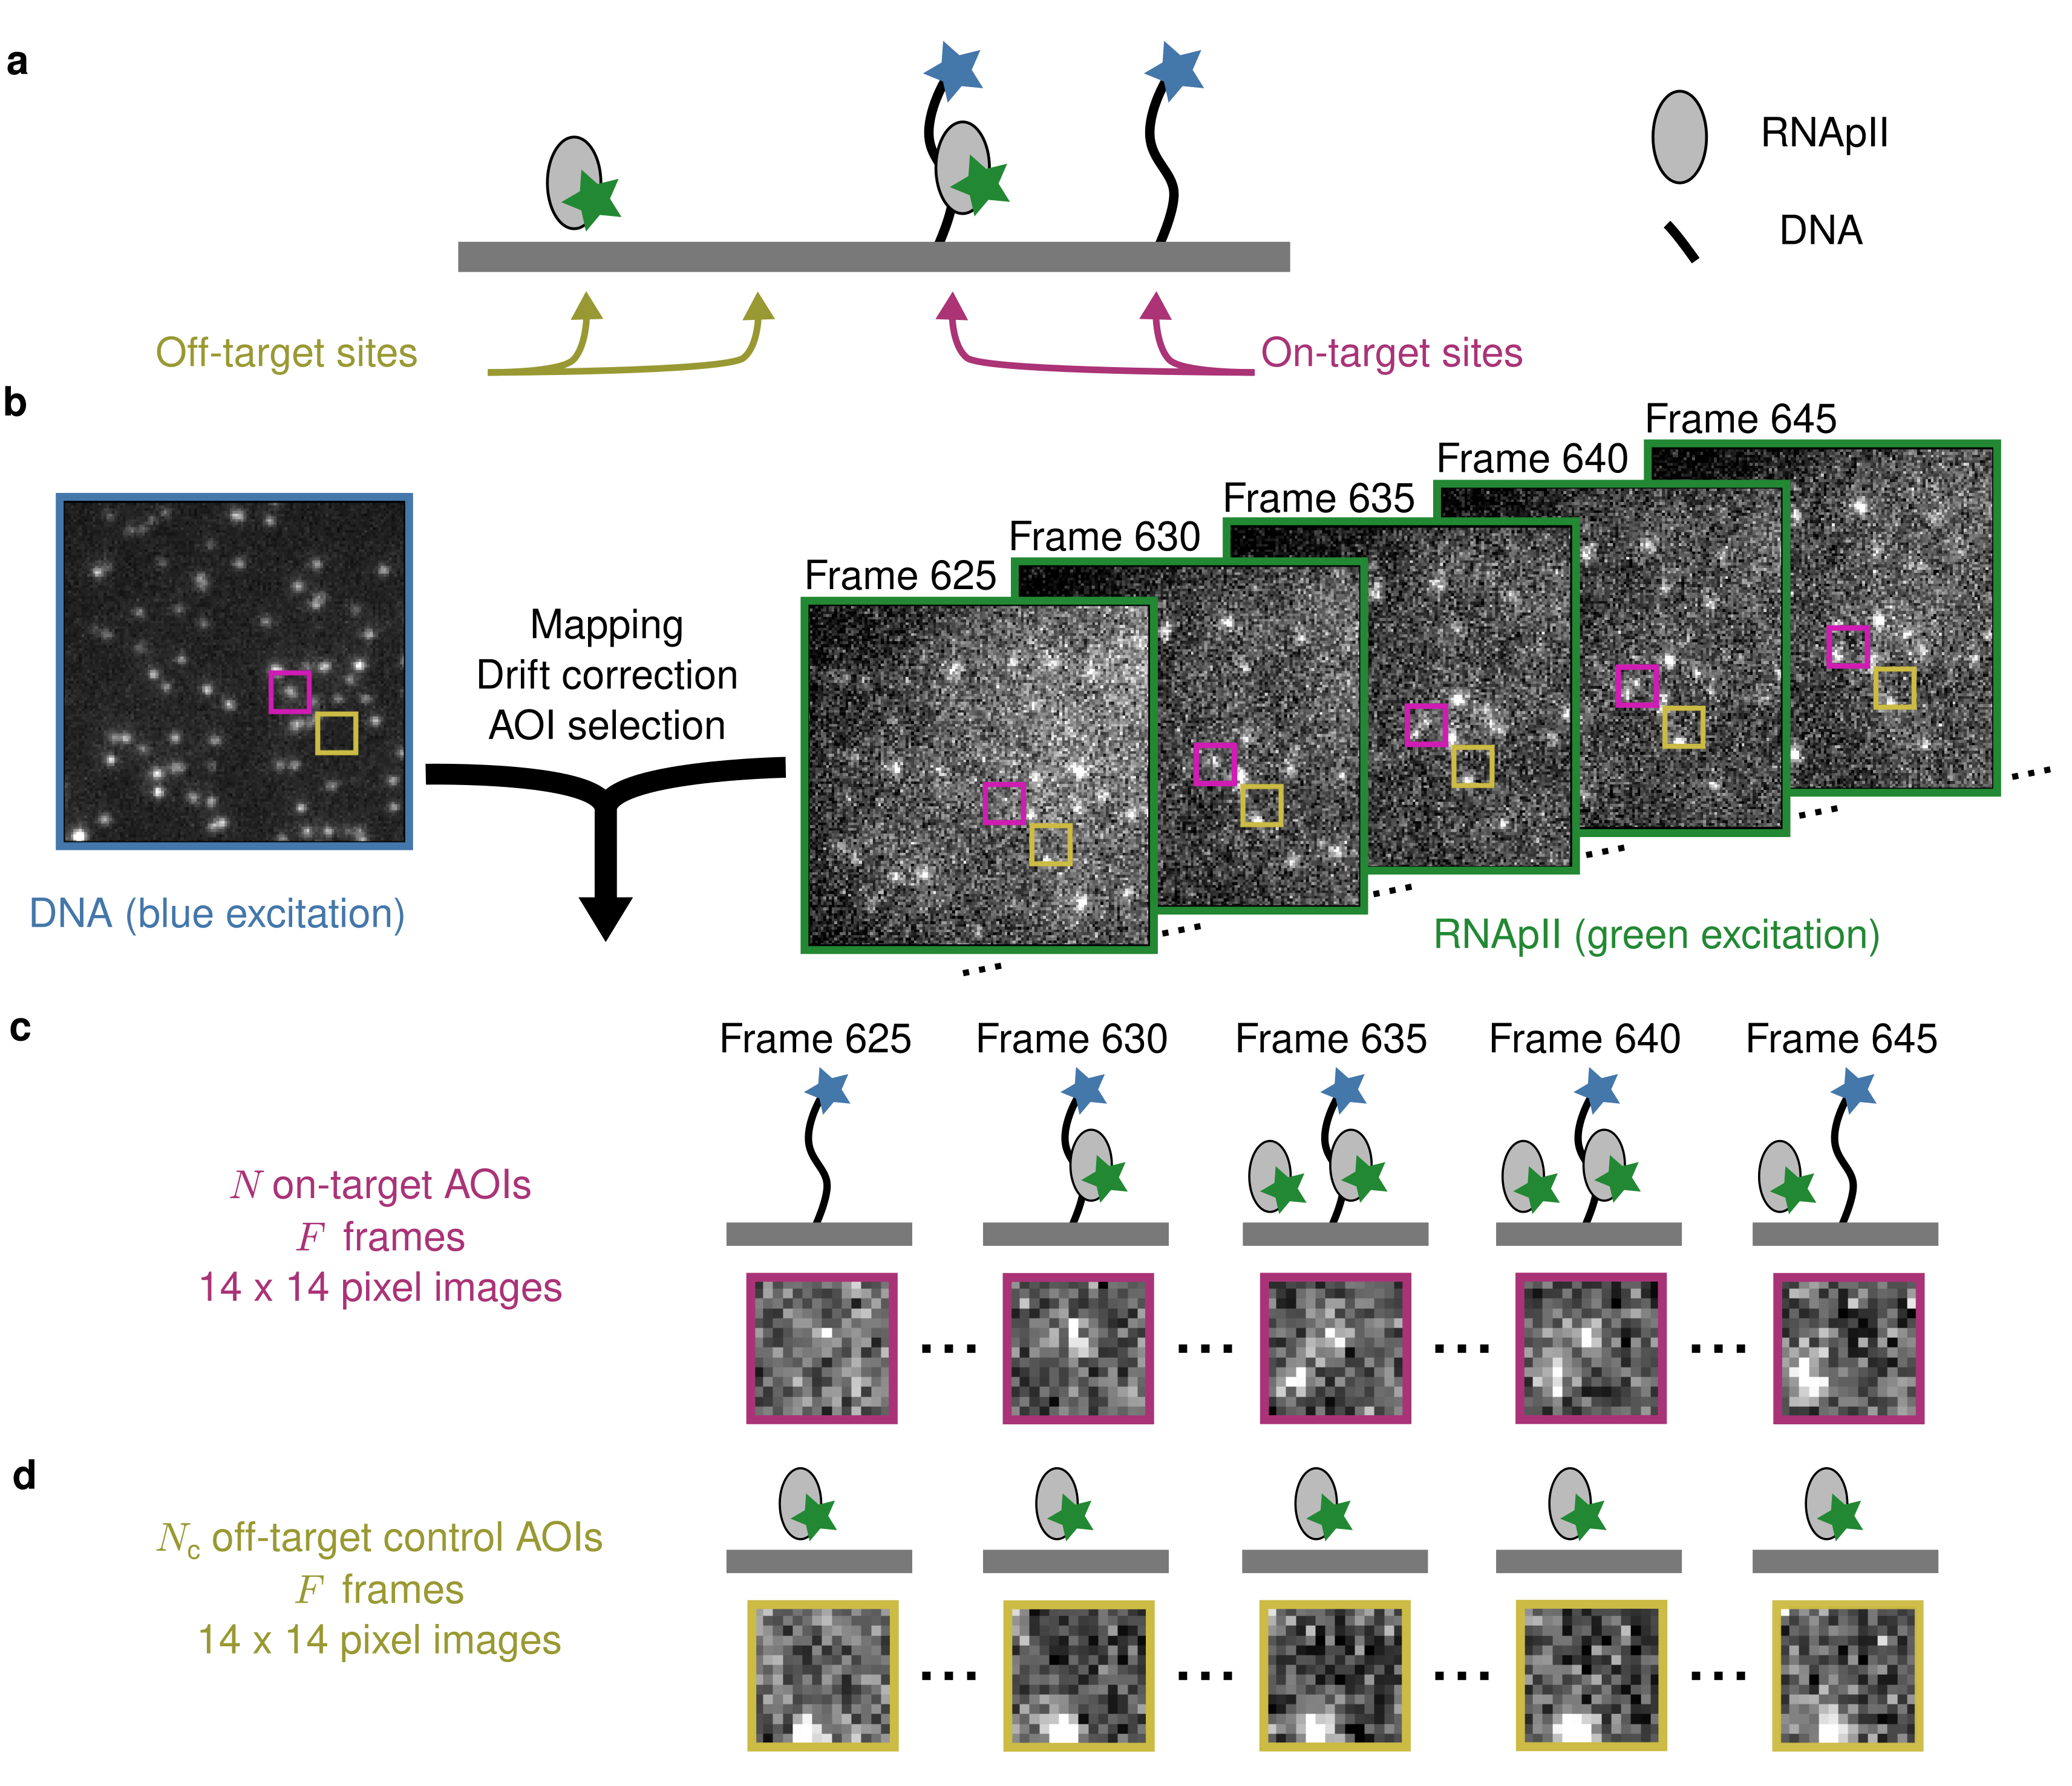
\includegraphics[width=75mm]{figures/figure1/figure1.png}
\captionsetup{labelformat=empty} % makes sure dummy caption is blank
\caption{} % add dummy caption - otherwise \label won't work and figure numbering will not count up
\label{fig1} % use \ref{fig1} to reference to this figure
\end{wrapfigure} % avoid blank space here
the interaction kinetics of RNA polymerase molecules with DNA. The key features of a CoSMoS experiment include: 1) One species of fluorescently labeled molecule (called the “target”) is tethered to the surface of the observation chamber. Target molecules are immobilized at a surface density sufficiently low that the mean nearest-neighbor distance is large relative to the point-spread function (i.e., the diffraction-limited spot size) of the microscope. 2) Molecules, each species labeled with a different dye color, are added to the solution over the surface, typically at concentrations $\leq 1 \mu$M. When these “binder” molecules are freely diffusing in solution, they are invisible in TIRF. In contrast, when they are bound to the target, single binder molecules are detected as discrete fluorescent spots. The combination of features 1 and 2 means that formation of an individual binder-target complex is detected as spot appearance; dissociation of a binder-target complex is detected as spot disappearance \cite{Friedman2006-kb, Friedman2015-nx}.

Effective data analysis is the major challenge in the use of the CoSMoS technique. The most basic task in CoSMoS data analysis is spot discrimination. The goal is to acquire information at each time point about whether a binder molecule fluorescence spot is observed at the image position of a target molecule (e.g., whether a co-localized green RNA polymerase is observed at the surface location of a blue DNA spot in Figure~\ref{fig1}B). Although CoSMoS images are conceptually simple -- they consist only of diffraction-limited fluorescent spots collected in several wavelength channels -- efficient analysis of the images is inherently challenging for several reasons. First, the number of photons emitted by a single fluorophore is limited by fluorophore photobleaching. Consequently, it is desirable to work at the lowest feasible excitation power in order to maximize the duration of experimental recordings and to efficiently capture relevant reaction events. Achieving sufficient time resolution divides the number of emitted photons between a larger number of images, often causing photon shot noise to dominate the data statistics. The required concentrations of fluorescently tagged molecules can sometimes create significant background noise \cite{Peng2018-ge, Van_Oijen2011-ig}, even with zero-mode waveguide instruments \cite{Chen2014-jd}. These technical difficulties result in CoSMoS images that frequently have low signal-to-noise (S/N) ratios, making discrimination of real fluorescent spots from noise a major challenge. Second, there are usually non-specific interactions of the binder molecule with the surface of the microscope slide, and these  artefacts can give rise to both false positive and false negative spot detections. These defects in analyzing spot colocalization interfere with the interpretation of CoSMoS data to measure reaction kinetics and interfere with reaching conclusions about molecular mechanisms.

Early CoSMoS spot detection methods were based on integrating the binder fluorescence intensity over small regions of the image (typically squares \SI{0.4}[\sim]{\um} on a side) centered on the location of the target molecule, and then using crossings of an intensity threshold to score binder molecule arrival and departure \cite{Friedman2015-nx}. However, integration discards data about the spatial distribution of intensity that can (and should) be used to distinguish an  authentic on-target spot from artefacts caused by noise or off-target binding.  More recently, improved methods \cite{Friedman2015-nx,Smith2019-yb} were developed that directly analyze the spatial distribution of intensities around the target molecule location to make a binary decision about the presence or absence of a binder spot at the target location.  However these are still heuristic methods that require tuning parameters based on arbitrary cut-offs of such quantities as spot intensity and proximity, and these methods fail to fully model the effects of non-specific binding.

In this paper, we describe a qualitatively different method for analysis of CoSMoS data and introduce a computer program, Tapqir, that implements the method. The method is based on an explicit, global model for CoSMoS image data and uses Bayesian inference to determine model parameters and associated uncertainties. The model incorporates physics-based shot noise, background noise, the size and shape of spots, and the presence of specifically and non-specifically bound molecules in the images. Importantly, instead of yielding a binary spot-/no-spot determination, the algorithm infers the probability of on target spot being present at each time point and target location; the calculated probability can then be used in subsequent analysis of the molecular mechanism. The method avoids use of arbitrary tuning parameters by using Bayesian methodology to formally learn and incorporate prior information about image formation and known properties of non-specific binding.  Since the method eliminates dependence on subjective threshold settings and includes built-in tools for statistical assessment of the validity of the results, it can be used effectively and accurately by non-expert practitioners. The Tapqir program is implemented in the Python-based probabilistic programming language Pyro, which facilitates implementation of new statistical models, scalability to large datasets, and efficient use of graphics processing unit (GPU)-based hardware for rapid parallel processing of data. 